% !TeX program = xelatex
% Projektová dokumentace — The Early Bowl
% Kompilace: xelatex projektova_dokumentace.tex  (2x kvůli obsahu a počtu stran)

\documentclass[12pt,a4paper]{article}

% --- Jazyk, typografie, fonty ---
\usepackage{fontspec}
\usepackage[czech]{babel}
\usepackage{microtype}
\usepackage{setspace}
\usepackage{ragged2e}
\usepackage{indentfirst}
\usepackage{etoolbox}

% Fonty podle MGO šablony: Caladea ≈ Cambria, Carlito ≈ Calibri
\setmainfont{Caladea}
\setsansfont{Carlito}
\newfontfamily\mgobodyfont{Caladea}
\newfontfamily\mgoheadingfont{Carlito}
\newfontfamily\mgotitlefont{Carlito}
\newfontfamily\mgofooterfont{Carlito}

\newcommand{\track}[2]{{\addfontfeatures{LetterSpace=#1}#2}}

% --- Rozměry stránky ---
\usepackage[
  a4paper,
  left=22mm,
  right=22mm,
  top=25mm,
  bottom=25mm,
  headheight=15pt,
  headsep=8mm,
  footskip=12mm
]{geometry}
\usepackage{tikz}
\usetikzlibrary{calc}
\usepackage[absolute,overlay]{textpos}

% --- Proměnné dokumentu ---
\newcommand{\typprace}{Závěrečný projekt}
\newcommand{\nazevprace}{The Early Bowl}
\newcommand{\podnazevprace}{snídaňová restaurace pro studenty a sportovce}
\newcommand{\autor}{Amélie Šamárková}
\newcommand{\skola}{Mendelovo gymnázium, Opava, příspěvková organizace}
\newcommand{\predmet}{informatika}
\newcommand{\misto}{Opava}
\newcommand{\rok}{2026}

% --- Odstavce ---
\onehalfspacing
\setlength{\parindent}{12mm}
\setlength{\parskip}{9pt}
\AtBeginDocument{\justifying}

\makeatletter
\patchcmd{\@afterheading}{\@afterindenttrue}{\@afterindentfalse}{}{}
\makeatother

% --- Záhlaví a zápatí ---
\usepackage{fancyhdr}
\usepackage{lastpage}
\pagestyle{fancy}
\fancyhf{}
\fancyhead[R]{{\mgobodyfont\itshape \typprace{} --- \nazevprace}}
\fancyfoot[C]{{\mgofooterfont\fontsize{10}{12}\selectfont \thepage/\pageref{LastPage}}}
\renewcommand{\headrulewidth}{0.4pt}
\renewcommand{\footrulewidth}{0.4pt}

\fancypagestyle{front}{%
  \fancyhf{}
  \renewcommand{\headrulewidth}{0pt}
  \renewcommand{\footrulewidth}{0pt}
}

% --- Nadpisy ---
\usepackage{titlesec}
\titleformat{\section}
  {\mgoheadingfont\fontsize{16}{19}\bfseries}
  {\thesection}{1.35em}{}
\titleformat{\subsection}
  {\mgoheadingfont\fontsize{14}{17}\bfseries}
  {\thesubsection}{1.2em}{}
\titleformat{\subsubsection}
  {\mgoheadingfont\fontsize{12}{14.5}\bfseries}
  {\thesubsubsection}{1.2em}{}

\titlespacing*{\section}{0pt}{18pt}{6pt}
\titlespacing*{\subsection}{0pt}{12pt}{3pt}
\titlespacing*{\subsubsection}{0pt}{9pt}{3pt}

% --- Obsah ---
\usepackage{tocloft}
\renewcommand{\contentsname}{Obsah}
\renewcommand{\cftsecleader}{\cftdotfill{\cftdotsep}}
\renewcommand{\cftsubsecleader}{\cftdotfill{\cftdotsep}}
\renewcommand{\cftsubsubsecleader}{\cftdotfill{\cftdotsep}}
\setlength{\cftsecnumwidth}{2.5em}
\setlength{\cftsubsecnumwidth}{3.2em}
\setlength{\cftsubsubsecnumwidth}{4.1em}
\setcounter{tocdepth}{2}
\setcounter{secnumdepth}{3}

\renewcommand{\cfttoctitlefont}{\mgoheadingfont\fontsize{16}{19}\bfseries}
\renewcommand{\cftsecfont}{\normalfont}
\renewcommand{\cftsecpagefont}{\normalfont}
\renewcommand{\cftsubsecfont}{\normalfont}
\renewcommand{\cftsubsecpagefont}{\normalfont}
\renewcommand{\cftsubsubsecfont}{\normalfont}
\renewcommand{\cftsubsubsecpagefont}{\normalfont}

% --- Seznamy ---
\usepackage{enumitem}
\setlist[itemize]{label=--, leftmargin=12mm, itemsep=0pt, topsep=3pt}
\setlist[enumerate]{leftmargin=12mm, itemsep=0pt, topsep=3pt}

% --- Obrázky, tabulky, odkazy ---
\usepackage{graphicx}
\usepackage{booktabs}
\usepackage{array}
\usepackage{tabularx}
\usepackage[hidelinks]{hyperref}
\usepackage{url}
\usepackage{csquotes}
\newcolumntype{Y}{>{\raggedright\arraybackslash}X}
\newcolumntype{R}{>{\raggedleft\arraybackslash}X}

% --- Pomocné příkazy ---
\newcommand{\blankpage}{\newpage\thispagestyle{front}\null\newpage}

\begin{document}

% =========================================================
% Titulní strana
% =========================================================
\thispagestyle{front}
\begin{titlepage}
\setlength{\TPHorizModule}{1mm}
\setlength{\TPVertModule}{1mm}

\begin{textblock*}{210mm}(0mm,25mm)
\centering {\mgobodyfont\fontsize{16}{19}\selectfont\mdseries \skola}
\end{textblock*}

\begin{textblock*}{210mm}(0mm,80mm)
\centering {\mgobodyfont\fontsize{16}{19}\selectfont\mdseries\track{11}{\autor}}
\end{textblock*}

\begin{textblock*}{210mm}(0mm,115mm)
\centering {\mgotitlefont\fontsize{28}{33}\selectfont\mdseries\track{8}{\nazevprace}}
\end{textblock*}

\begin{textblock*}{210mm}(0mm,129mm)
\centering {\mgotitlefont\fontsize{16}{19}\selectfont\mdseries\track{14}{\podnazevprace}}
\end{textblock*}

\begin{textblock*}{210mm}(0mm,163mm)
\centering {\mgobodyfont\fontsize{16}{19}\selectfont\mdseries\track{6}{\typprace{} z~předmětu \predmet}}
\end{textblock*}

\begin{textblock*}{210mm}(0mm,256mm)
\centering {\mgobodyfont\fontsize{16}{19}\selectfont\mdseries\track{12}{\misto{} \rok}}
\end{textblock*}

\end{titlepage}

\blankpage

% =========================================================
% Prohlášení
% =========================================================
\thispagestyle{front}
\vspace*{12cm}
Prohlašuji, že jsem tento závěrečný projekt vypracovala samostatně na základě uvedených pramenů a literatury. Web, ilustrace, fotografie a text dokumentace jsem vytvořila vlastními silami s pomocí výslovně uvedených AI nástrojů.

\vspace{1.5cm}
\noindent V~\misto{} dne \today \hfill Podpis: \rule{45mm}{0.4pt}

\blankpage

% =========================================================
% Obsah
% =========================================================
\thispagestyle{front}
\tableofcontents
\newpage

% =========================================================
% Úvod
% =========================================================
\section*{Úvod}
\addcontentsline{toc}{section}{Úvod}

Cílem projektu bylo navrhnout fiktivní snídaňovou restauraci \textbf{The Early Bowl} a vytvořit pro ni kompletní webovou prezentaci. Restaurace má sídlit v~centru Opavy (Náměstí Republiky 159/10, OD Stará Breda), otevřeno 6:00--13:30, a~cílí na středoškolské a~vysokoškolské studenty a~sportovce z~fitnescentra. Web slouží jako digitální vizitka: menu, příběh značky, kontakt a~otvírací doba. Tato dokumentace popisuje teoretická východiska tvorby webu i~konkrétní cestu, kterou projekt prošel.

Projekt vědomě následuje princip \textbf{spec-driven development} -- nejdřív vznikla pořádná dokumentace značky a~specifikace webu (paleta, fonty, persony, datový model menu), teprve potom z~ní AI nástroje generovaly samotný kód. AI je tu výkonný spolupracovník, ne náhrada za promyšlený záměr.

Živý web:\\
\url{https://ameliesam.github.io/the-early-bowl/}

\noindent Zdrojové soubory:\\
\url{https://github.com/AmelieSam/the-early-bowl}

% =========================================================
% A. TEORETICKÁ ČÁST
% =========================================================
\section{Webové technologie}

\subsection{Co je web a jak funguje}

Webová stránka je soubor (nejčastěji typu HTML), který si počítač uživatele stáhne ze vzdáleného serveru a~prohlížeč jej zobrazí. Aby uživatel věděl, kam má jít, slouží \textbf{doména} -- lidsky čitelná adresa typu \texttt{theearlybowl.cz}. Doména se přes systém DNS překládá na IP adresu konkrétního serveru.

\textbf{Hosting} je placená nebo bezplatná služba, která provozuje server a~drží na něm soubory webu dostupné nepřetržitě. V~tomto projektu jsme zvolili \textbf{GitHub Pages} -- bezplatný hosting přímo z~verzovaného repozitáře, který automaticky zajišťuje šifrované HTTPS spojení. Web tak běží na generické adrese \texttt{ameliesam.github.io/the-early-bowl/} bez nutnosti platit vlastní doménu (řádově 400~Kč/rok).

\subsection{Tři základní jazyky webu}

\begin{itemize}
  \item \textbf{HTML} (HyperText Markup Language) -- definuje \emph{strukturu} stránky (nadpisy, odstavce, obrázky, odkazy).
  \item \textbf{CSS} (Cascading Style Sheets) -- definuje \emph{vzhled} (barvy, fonty, rozložení, responzivitu).
  \item \textbf{JavaScript} -- přidává \emph{interaktivitu} (rozbalovací menu, kopírování ID do schránky).
\end{itemize}

Pro tento projekt jsme zvolili „čistý" stack bez frameworků jako React nebo WordPress. Pět statických stránek se totiž obejde bez složitých nástrojů, web je rychlejší, levnější a~má méně bezpečnostních rizik.

\subsection{Co je CMS a proč jsme ho nepoužili}

\textbf{CMS} (Content Management System) jako WordPress, Webnode nebo Shoptet je hotová „továrna na weby" -- uživatel klikáním sestaví stránku, aniž by psal kód. Výhodou je rychlost a~komfort, nevýhodou závislost na platformě a~měsíční poplatky. Naše statické řešení má navíc \textbf{nulové náklady na provoz a~správu} (žádný měsíční hosting, žádné aktualizace pluginů, žádné bezpečnostní záplaty) -- to je s~redakčními systémy a~placenými hostingy nesrovnatelná výhoda.

\subsection{Responzivita}

Více než polovina uživatelů dnes prohlíží web na mobilu. \textbf{Responzivní design} znamená, že web sám přizpůsobí rozložení velikosti obrazovky -- na telefonu se mění menu na rozbalovací, sloupce se skládají pod sebe a~fotky se zmenšují tak, aby se nemusely posouvat do stran.

\section{Základy UX/UI}

\textbf{UX} (User Experience) je celkový zážitek uživatele -- jestli najde, co hledá, jestli mu to dává smysl, jestli se mu chce vrátit. \textbf{UI} (User Interface) je vizuální vrstva -- barvy, tlačítka, typografie. UX se ptá „funguje to dobře?", UI „vypadá to dobře?". Dobrý web potřebuje obojí.

\subsection{Co dělá web přehledným}

\begin{enumerate}[label=\arabic*.]
  \item \textbf{Jasná navigace} -- uživatel musí kdykoliv vědět, kde je a~jak se dostane domů. V~našem webu je horní menu (Menu, O~nás, Kontakt) na každé stránce stejné.
  \item \textbf{Vizuální hierarchie} -- důležité prvky (cena, tlačítko „kontaktovat") musí být na první pohled výraznější než vedlejší informace. Realizuje se velikostí, barvou a~prostorem.
  \item \textbf{Pravidlo tří kliků} -- uživatel by měl ke kterékoliv informaci dorazit nejvýše třemi kliky. U~pětistránkového webu je to triviální.
  \item \textbf{Kontrast a čitelnost} -- text musí mít proti pozadí dostatečný kontrast, aby se dal pohodlně přečíst i~na mobilu na slunci. Naše hnědé písmo na smetanovém pozadí ho má s~rezervou.
  \item \textbf{Rychlost} -- pokud se stránka načítá déle než 3~sekundy, polovina návštěvníků odejde. Proto jsme obrázky komprimovali do formátu WebP, hero foto kleslo z~1{,}1~MB na 73~kB.
\end{enumerate}

\subsection{Proč je uživatelská přívětivost důležitá}

Zákazník nepřišel obdivovat náš web -- přišel se rozhodnout, jestli si u~nás dá snídani. Pokud do deseti sekund nenajde otvírací dobu, adresu a~ukázku menu, odejde ke konkurenci. Dobrý UX je tedy přímo měřitelný v~tržbě.

\section{Bezpečnost a legislativa}

\subsection{GDPR}

Každý web, který sbírá osobní údaje občanů EU (jméno, e-mail, IP adresu přes analytiku), musí mít zpracované zásady zpracování osobních údajů a~často i~cookie lištu. Náš web tuto situaci elegantně řeší tím, že \textbf{nesbírá žádné osobní údaje}: nemá kontaktní formulář, žádné analytics, žádné sledovací cookies. Návštěvník nemusí nic odklikávat, GDPR ho v~podstatě nemůže ohrozit. Tento záměr -- „webové prostředí bez třecích ploch" -- je sám o~sobě v~roce 2026 odlišujícím znakem.

\subsection{Obchodní podmínky}

E-shop podle českého práva potřebuje uvedené obchodní podmínky (právo na odstoupení do 14~dnů, reklamační řád, popis dodání). Naše stránka \texttt{podminky.html} je v~zúžené verzi -- restaurace je fyzický provoz bez online prodeje, takže obchodní podmínky se v~praxi smrskávají na informace o~provozovateli, vyloučení odpovědnosti a~popis toho, že web neslouží jako e-shop a~žádné platby přes něj neprobíhají.

\subsection{Zabezpečení plateb a autorská práva}

Pokud by web zpracovával platby, je naprostou nutností HTTPS (šifrované spojení) a~integrace s~certifikovanou platební bránou (GoPay, ComGate, Stripe). Naše restaurace přijímá platby fyzicky na pokladně, online platby tedy zatím neřešíme. HTTPS na webu přesto máme -- zajišťuje ho automaticky GitHub Pages a~zvyšuje důvěryhodnost stránky.

Veškerý obsah na webu -- texty, ilustrace, video -- vytvořila autorka projektu, případně byl vygenerován AI nástroji na základě vlastních zadání. Žádné cizí fotografie ani stock obrázky nepoužíváme. Použité fonty (Baloo~2, Quicksand) jsou pod otevřenou licencí SIL Open Font License a~jejich komerční použití je zdarma.

% =========================================================
% B. PRAKTICKÁ ČÁST
% =========================================================
\section{Příběh značky}

The Early Bowl se zrodila z~osobní zkušenosti. Hledali jsme v~Opavě místo, kde si dáme pořádnou snídani, a~nenašli jsme. Většina kaváren v~centru otevírá až po osmé, restaurace až po desáté, a~pekárny mají sice levné, ale jednotvárné a~nezdravé pečivo. Studenti, kteří přijdou na ranní přednášku na lačno, sportovci po cvičení ani lidé jdoucí do ranní směny nemají kam zajít.

Tak vznikl koncept \emph{„misky optimismu pro ranní lidi"} -- fyzické místo otevřené už od šesti hodin ráno, kde si zákazník během pěti minut objedná zdravou, čerstvou snídani za přijatelnou cenu a~nemusí kvůli ní vstávat hodinu předem. Tři pilíře značky znějí jednoduše: \textbf{rychlé, zdravé, dostupné}. Každé rozhodnutí -- od ceníku přes vizuální styl až po komunikaci na Instagramu -- musí jeden z~těchto pilířů podpořit. Nejde tedy o~„další moderní bistro", ale o~cílený zásah do jasně definované mezery na opavském trhu.

\section{Vizuální identita}

Vizuální styl značky stojí na \textbf{logu} (keramická miska s~jogurtem, granolou a~ovocem), které jsem vytvořila nejprve ručně a~poté přes Google Gemini. Z~loga jsme odvodili celý design systém -- paletu, kresebný styl ilustrací jídel i~typografii.

\subsection{Paleta a její psychologie}

\begin{itemize}
  \item \textbf{Smetanová} (\texttt{\#FAF6EE}) jako hlavní pozadí. Místo „nemocniční bílé" působí teple, evokuje mléko, jogurt, ranní světlo.
  \item \textbf{Čokoládová hnědá} (\texttt{\#7A5843}) pro texty a~kontury -- barva pražené kávy, granoly, sourdough. Působí důvěryhodně, „doma upečeně".
  \item \textbf{Jahodová červená} (\texttt{\#E3413B}) pro tlačítka a~akce -- energie, chuť, optimismus, přitahuje pozornost.
  \item \textbf{Borůvková modrá} (\texttt{\#4B679B}) pro odkazy.
  \item \textbf{Medová žlutá} (\texttt{\#F3C46B}) pro důležité informace.
  \item \textbf{Listová zelená} (\texttt{\#7FA86B}) pro „healthy" ikony (vegan, bez lepku).
\end{itemize}

Paleta vědomě \emph{nepoužívá} neonové ani studené odstíny -- ty patří fastfoodovým řetězcům a~fitness aplikacím. Snídaňová restaurace musí vyvolávat teplo, klid a~péči.

\subsection{Typografie}

Pro nadpisy je zvolen font \textbf{Baloo~2} -- zaoblený, tučný, hravý, který ladí s~ručně kresleným charakterem loga. Pro tělo textu \textbf{Quicksand} -- geometrický, dobře čitelný, mírně zaoblený. Oba fonty jsou bezplatné na Google Fonts.

Při testování fontů se ukázal důležitý detail. Původně zvolená \textbf{Fredoka} sice vypadala dobře v~angličtině, ale neobsahuje vlastní glyfy českých háčků (\textit{ě č ř š ž}). Prohlížeč si je dotahoval ze systémového fontu, takže háčky byly tenké a~ke zbytku slova stylově nesedící. Defekt jsme odhalili vizuálním testem v~prohlížeči (nástroj Playwright + screenshot) a~vyměnili font za Baloo~2, který diakritiku zvládá. Poučení: u~každého nového fontu zkontrolovat český pangram, ne se spoléhat na to, co tvrdí Google Fonts.

\section{Cenotvorba}

\subsection{Filozofie ceníku}

Záměrně držíme \textbf{jednoduchý dvouhladinový ceník}: 90 nebo 110~Kč u~jídel, 25--55~Kč u~nápojů. Zákazník se nemusí rozhodovat podle ceny, ale podle toho, na~co má chuť. Jednoduchost je sama o~sobě hodnotou značky.

\subsection{Náklady a marže}

\begin{table}[h]
  \centering
  \caption{Kalkulace food costu jednotlivých položek menu}
  \begin{tabularx}{\textwidth}{Y r r r}
    \toprule
    \textbf{Položka} & \textbf{Cena} & \textbf{Suroviny} & \textbf{Food cost} \\
    \midrule
    Voda s citronem (N1) & 25 Kč & 3 Kč & 12 \% \\
    Čaj (N3) & 35 Kč & 5 Kč & 14 \% \\
    Čerstvě mačkaný pomerančový džus (N2) & 55 Kč & 15 Kč & 27 \% \\
    Denní polévka (P1) & 65 Kč & 18 Kč & 28 \% \\
    Yogurt Bowl (S1) & 90 Kč & 25 Kč & 28 \% \\
    Teplá kaše (S2) & 90 Kč & 15 Kč & 17 \% \\
    Vajíčka s toastem (M2) & 90 Kč & 22 Kč & 24 \% \\
    Toast Caprese (M4) & 90 Kč & 28 Kč & 31 \% \\
    Avokádový toast s lososem (M1) $\star$ & 110 Kč & 38 Kč & 35 \% \\
    Vajíčka s avokádem a slaninou (M3) $\star$ & 110 Kč & 38 Kč & 35 \% \\
    \bottomrule
  \end{tabularx}

  \vspace{2pt}
  \footnotesize $\star$~=~prémiové „anchor" položky, vědomě vyšší food cost.
  \label{tab:foodcost}
\end{table}

\subsection{Bod zlomu}

Měsíční fixní a~kvazi-fixní náklady (mzdy, nájem, energie, marketing) činí přibližně 75\,000~Kč. Při průměrné jednotkové marži 111~Kč na zákazníka je bod zlomu \textbf{23~zákazníků denně}. Cílový scénář 25~zákazníků/den znamená zisk přibližně 7\,500~Kč/měsíc. Realisticky tomu předchází 4--6 měsíců provozní ztráty, pro start je tedy potřeba rezerva přibližně 300\,000~Kč. Kapitál lze doplnit dotací Statutárního města Opavy (až 100\,000~Kč) nebo zvýhodněným úvěrem Národní rozvojové banky.

\section{Cílová skupina}

Cílíme na \textbf{tři primární persony}, které dohromady vytvoří přibližně 80~\% očekávaného obratu.

\begin{itemize}
  \item \textbf{Tereza (21), studentka Slezské univerzity} -- bydlí 10~minut chůze od centra, má ranní přednášku v~8:00, prázdnou lednici a~nestihne menzu. Triggerem je IG story od kamarádky nebo leták v~MHD. Vysoká frekvence návštěv (3--4× týdně), nízká útrata (přibližně 125~Kč).
  \item \textbf{Michal (28), sportovec po ranním tréninku} -- cvičí v~5:45, v~7:00 hladový po sprše. Chce pořádnou snídani s~proteinem, ne shake. Trigger: plakát v~gymu. Vysoká útrata (přibližně 165~Kč), 2--3× týdně.
  \item \textbf{Jana (35), pracující na ranní směně} -- vezme si „něco po cestě", ale nechce croissant z~benzínky. Trigger: Google search „snídaně Opava". Střední frekvence, velmi loajální zákaznice.
\end{itemize}

Sekundárně cílíme na \textbf{středoškoláky} -- ti často nesnídají vůbec (ráno spěch, peníze v~kapse, nechuť k~pekárně) a~jsou navíc TikTok publikem a~přirozenými brand evangelisty. O~víkendech doplňují cílovku místní rodiče s~dětmi.

\section{Marketingový plán}

Marketingový rozpočet je vědomě nízký -- 1\,750~Kč měsíčně. To vylučuje placené reklamy i~velké influencery. Vsázíme na \textbf{organický růst skrz brand a~lokální komunitu}.

\subsection{Online kanály}

Primárním kanálem je \textbf{Instagram} -- přibližně 70~\% marketingové pozornosti. Pravidelný kalendář: neděle = týdenní menu, středa = příběh suroviny, pátek = behind-the-scenes; denní stories s~aktuální polévkou a~děním v~provozu. Cíl po třech měsících: 200+ sledujících, engagement~$>5$~\%. Web slouží jako digitální vizitka a~referenční bod pro Google search, ne jako akviziční kanál. Facebook je pouze automaticky zrcadlený obsah z~Instagramu.

\subsection{Offline kanály}

Plakát formátu A3 v~partnerském fitness centru výměnou za slevu 10~\% pro jeho členy. Distribuce letáčků formátu A6 s~QR~kódem před fakultou Slezské univerzity a~v~MHD na trase ke školám (500~kusů pro start, přibližně 750~Kč). Tisková zpráva měsíc po otevření do regionálních médií \emph{Hláska} a~\emph{Opavský deník} se sdělením „mladá podnikatelka, snídaňová restaurace pro studenty".

\subsection{Lokální SEO}

Google Business Profile s~otvírací dobou, fotkami a~aktivním sběrem recenzí (cíl: 30+ recenzí, průměr alespoň 4{,}5~hvězdy za tři měsíce). Web optimalizovaný na long-tail dotazy „snídaně Opava", „avokádový toast Opava", „otevřeno od 6 ráno Opava" -- konkurence na tyto dotazy je v~Opavě minimální, reálná šance na první stránku Google během dvou až tří měsíců.

\section{Reflexe tvorby}

\subsection{Co bylo nejnáročnější}

Největším úkolem nebyla samotná tvorba kódu, ale \textbf{vytvoření kvalitního zadání pro AI nástroje} -- tedy přesně to, čemu se říká \emph{spec-driven development}. První pokusy s~nástrojem Google Stitch (generátor návrhů webu) selhaly, protože jsem mu dala slabý kontext -- výstupy byly generické a~nepoužitelné. Free verze Gemini a~GitHub Copilotu rovněž nestačily. Ukázalo se, že platí pravidlo \emph{„garbage in, garbage out"}: nejdřív musí vzniknout pořádná specifikace (paleta, fonty, příběh, persony, datový model menu) a~teprve pak má smysl pustit AI ke generování webu.

\subsection{Placené versus bezplatné AI nástroje}

Velkým poznatkem bylo, jak zásadní rozdíl je mezi \textbf{bezplatnými} a~\textbf{placenými} verzemi AI nástrojů. Free verze Gemini, GitHub Copilotu a~podobné jsou užitečné na rychlé pokusy, ale pro reálnou práci s~rozsáhlejším kontextem (celý projektový spec, několik souborů zároveň) selhávají -- krátí kontext, halucinují, vyrábějí generický výstup. Placené verze (Claude Code s~tarifem Max, ChatGPT Plus, Gemini Advanced) za řádově 500--2\,000~Kč/měsíc poskytují kvalitativně jinou úroveň práce. \textbf{Doporučení:} kdo to s~podobným projektem myslí vážně, ať si předplatí alespoň jeden profesionální AI nástroj. Vrátí se to v~desetinásobku času.

\subsection{Co mě naopak bavilo}

Spolupráce s~\textbf{Claude Code} byla zážitkem podobným tomu, kdy člověk pracuje s~velmi pečlivým kolegou, který nezapomíná na detaily. Když jsem chtěla změnit cenu jedné položky, automaticky se přepočítaly food cost, marže i~bod zlomu. Když jsem požádala o~test diakritiky, navrhl, abychom rovnou vytvořili srovnávací stránku se sedmi fonty a~porovnali je vizuálně.

Bavilo mě také promýšlení detailů, které normální zákazník nepozná, ale tvoří celkovou kvalitu: proč použít smetanovou místo bílé (teplejší), proč zmenšit porci lososa z~50 na 40~g a~zato ji lépe naservírovat (lepší marže bez ztráty vnímané hodnoty), proč ID položek na kartě udělat klikatelné (klik~=~kopírování do schránky pro snadnou telefonickou objednávku).

\subsection{Co bych udělala jinak}

Nejdřív bych investovala víc času do dokumentace značky a~teprve potom začala stavět web. Polovinu věcí jsem přepisovala, protože jsem zjistila, že produktový a~designový dokument si na začátku přímo odporovaly (zelená paleta versus smetanovo-hnědá). Také bych se dřív naučila pracovat s~verzováním v~Gitu -- uvědomila jsem si jeho cenu až poté, co jsem mohla bezpečně experimentovat se změnami.

\section{Screenshot úvodní stránky}

Pro ilustraci responzivního chování webu zachycuje obrázek~\ref{fig:hero-mobile} úvodní stránku v~mobilním zobrazení (viewport iPhone 13~Pro, 390$\times$844, DPR~3). Screenshot byl pořízen automatizovaně přes nástroj Playwright.

\begin{figure}[h]
  \centering
  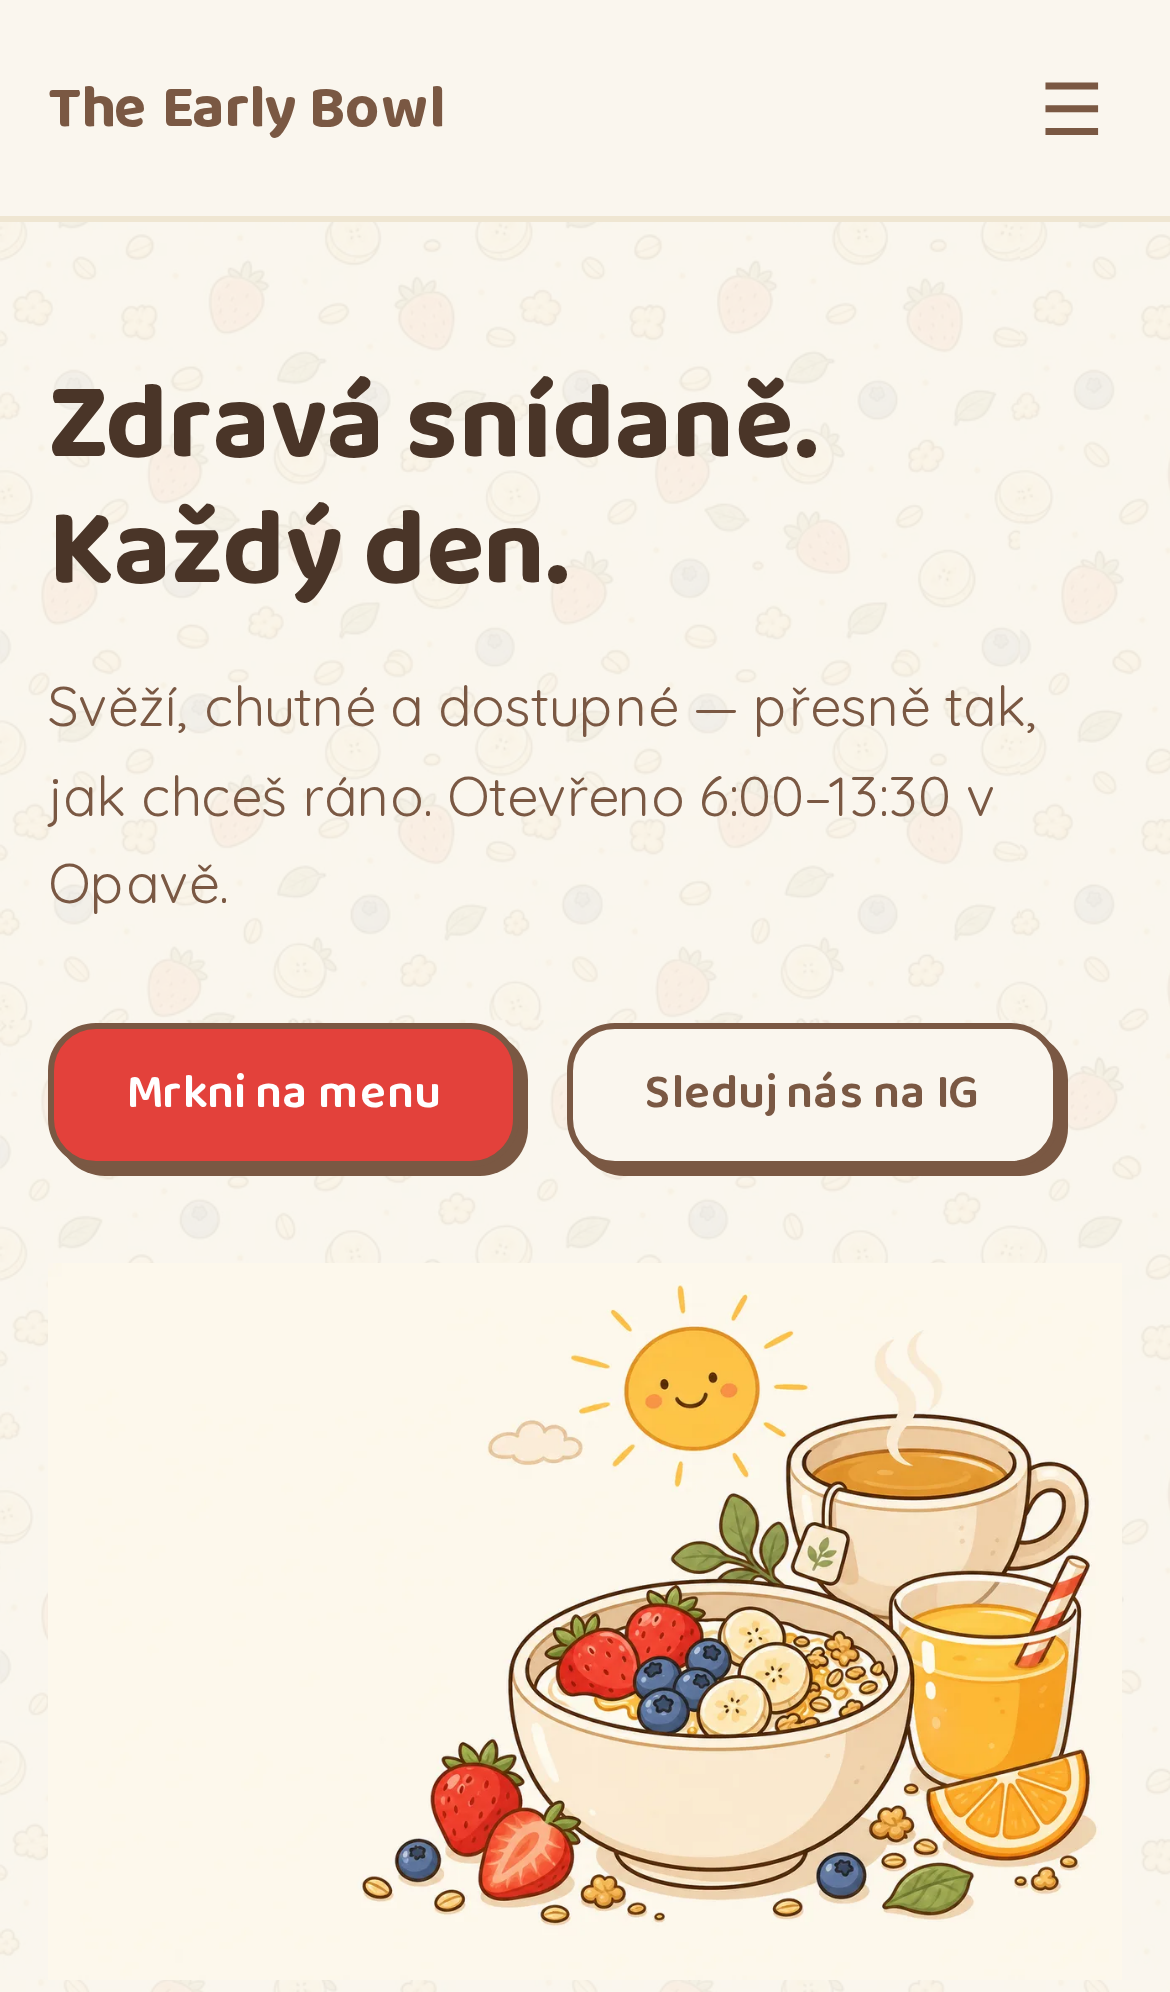
\includegraphics[width=0.42\textwidth]{screenshot-mobile.png}
  \caption{Úvodní stránka v~mobilním zobrazení -- logo, hero claim „Zdravá snídaně. Každý den.", tlačítka „Mrkni na menu" a~„Sleduj nás na IG" a~brandová ilustrace misky.}
  \label{fig:hero-mobile}
\end{figure}

\section{Použité zdroje a nástroje}

\subsection{Zjednodušený pracovní postup}

\begin{enumerate}[label=\arabic*.]
  \item \textbf{Idea a koncept} (duben 2026) -- nápad snídaňové restaurace; ověření dostupnosti názvu; první návrhy loga v~Google Gemini.
  \item \textbf{Konzultace s otcem} (s~IT zkušeností a~znalcem AI nástrojů) -- celá konzultace nahrána na diktafon, převod do textového zápisu pak vytvořen pomocí NotebookLM. Dokument \texttt{zapis\_konzultace.md} se v~celém projektu stal stabilní „kotvou".
  \item \textbf{Strukturování kontextu (spec-driven development)} -- sepsání produktového požadavku, design systému a~brandového příběhu jako Markdown dokumentů ve VS~Code. Tato fáze trvala záměrně několik dní, protože všechno další z~ní stavělo.
  \item \textbf{Generování ilustrací} -- 21~obrázků (jídla, hero, OG obrázek, 404 stránka, dietní ikony, favicon, logo varianty) vygenerováno přes textové prompty v~nástroji Codex podle stylového bloku odvozeného z~loga.
  \item \textbf{Tvorba webu} -- pět HTML stránek, CSS s~designovými tokeny, vanilla JavaScript pro interaktivitu. Veškerý kód vznikal v~dialogu s~nástrojem Claude Code; já zadávala požadavky a~kontrolovala výstup v~prohlížeči.
  \item \textbf{Datový model menu} -- položky menu uloženy v~souboru \texttt{menu.yaml} jako jediný zdroj pravdy. Web čte YAML přímo v~prohlížeči přes vlastní mini-parser; jakákoliv změna položky či ceny stačí na jediném místě.
  \item \textbf{Vizuální kontrola} -- automatizovaný rendering stránek přes Playwright (skriptovaný prohlížeč) na desktop i~mobil, nula JavaScriptových chyb, nula selhaných requestů.
  \item \textbf{Generování propagačního videa} -- top-down příprava Yogurt Bowl ve formátu vhodném pro Instagram, vygenerováno v~Google Gemini Veo z~textového promptu uloženého ve zdrojích.
  \item \textbf{Nahrání na hosting} -- verzování přes Git, push do GitHub repozitáře, automatický deploy z~větve \texttt{main}, složky \texttt{/docs} přes službu GitHub Pages.
  \item \textbf{Projektová dokumentace} -- Markdown text převedený do PDF přes LaTeX šablonu ve stylu Mendelova gymnázia Opava.
\end{enumerate}

\subsection{Klíčové nástroje a platformy}

\begin{itemize}
  \item \textbf{VS Code} -- vývojové prostředí (editor), v~němž vznikal veškerý kód i~dokumentace.
  \item \textbf{Git + GitHub} -- verzování souborů, vzdálený repozitář, hosting webu (GitHub Pages).
  \item \textbf{Claude Code} (model Opus 4.7) -- hlavní AI nástroj, který v~dialogu generoval kód, kontroloval konzistenci dokumentů, hledal chyby (diakritika) a~počítal cenotvorbu.
  \item \textbf{Codex} (OpenAI ChatGPT Images) -- generování 21~brandových ilustrací podle stylového promptu.
  \item \textbf{Google Gemini Veo} -- generování propagačního videa přípravy Yogurt Bowl.
  \item \textbf{Google Gemini} (raná fáze) -- první návrhy loga.
  \item \textbf{NotebookLM} -- zpracování briefu a~kontextu v~ideové fázi.
  \item \textbf{Playwright} (skriptovaný Chromium prohlížeč) -- vizuální kontrola webu, test diakritiky, automatizované screenshoty na desktopu i~mobilu.
  \item \textbf{Google Fonts} -- bezplatné fonty Baloo~2 a~Quicksand.
  \item \textbf{Google Maps Embed} -- mapa lokace na stránce Kontakt.
  \item \textbf{GitHub Pages} -- bezplatný hosting webu s~HTTPS.
  \item \textbf{LaTeX (XeLaTeX)} -- sazba této projektové dokumentace do PDF podle šablony Mendelova gymnázia Opava.
\end{itemize}

\subsection{Slepé uličky, ze kterých jsme se poučili}

\begin{itemize}
  \item \textbf{Google Stitch} -- generátor návrhů webu. Bez kvalitního kontextu dával jen šedivé generické šablony. Poučení: kvalita výstupu AI je rovna kvalitě vstupu.
  \item \textbf{Webnode / Shoptet} (zvažováno na začátku) -- pohodlné, ale neumožnily by plnou kontrolu nad vzhledem značky a~vlastním stylem.
  \item \textbf{HeyGen Hyperframes} (původně plánováno pro video) -- zbytečně složitá HTML$\rightarrow$video pipeline. Nahrazeno přímým textovým zadáním do Gemini Veo.
  \item \textbf{Cloudflare Pages} (původně zvolený hosting) -- nahrazeno GitHub Pages kvůli jednoduchosti a~integraci s~repozitářem.
\end{itemize}

% =========================================================
% Závěr
% =========================================================
\section*{Závěr}
\addcontentsline{toc}{section}{Závěr}

Projekt The Early Bowl ukázal, že i~středoškolský studentský projekt může mít produkční kvalitu -- pokud se začne pořádnou dokumentací značky a~teprve potom se sáhne po nástrojích. AI nástroje (Claude Code, Codex, Gemini Veo) celý vývoj radikálně zrychlily, ale samy o~sobě by nic nevyřešily: každý jejich výstup musel projít lidskou kontrolou a~navazoval na pečlivě promyšlený kontext. Web je živý na adrese \url{https://ameliesam.github.io/the-early-bowl/} a~slouží jako vizuální i~obsahová prezentace fiktivního, ale poctivě promyšleného opavského podnikatelského záměru.

\section*{Použité zdroje a nástroje}
\addcontentsline{toc}{section}{Použité zdroje a nástroje}

\begin{thebibliography}{9}
  \bibitem{claude}
  Anthropic. \textit{Claude Code} (model Opus 4.7). Dostupné z:\\
  \url{https://claude.com/claude-code}

  \bibitem{codex}
  OpenAI. \textit{ChatGPT (Codex, ChatGPT Images)}. Dostupné z:\\
  \url{https://chatgpt.com}

  \bibitem{gemini}
  Google. \textit{Gemini, Gemini Veo, NotebookLM}. Dostupné z:\\
  \url{https://gemini.google.com}

  \bibitem{vscode}
  Microsoft. \textit{Visual Studio Code}. Dostupné z:\\
  \url{https://code.visualstudio.com}

  \bibitem{github}
  GitHub, Inc. \textit{GitHub a GitHub Pages}. Dostupné z:\\
  \url{https://github.com}

  \bibitem{googlefonts}
  Google. \textit{Google Fonts -- Baloo~2, Quicksand}. Dostupné z:\\
  \url{https://fonts.google.com}

  \bibitem{playwright}
  Microsoft. \textit{Playwright -- end-to-end testing for modern web apps}. Dostupné z:\\
  \url{https://playwright.dev}

  \bibitem{repo}
  ŠAMÁRKOVÁ, Amélie. \textit{The Early Bowl -- zdrojové soubory projektu}. GitHub, 2026. Dostupné z:\\
  \url{https://github.com/AmelieSam/the-early-bowl}
\end{thebibliography}

\end{document}
